\documentclass[tt1]{penoverslag}

%%% PACKAGES
\usepackage{lipsum}


\begin{document}

\team{Zilver} % teamkleur
\members{Sam Gielis\\
         Sophie Marien\\
         Toon Nolten\\
         Nele Rober\\
         Gerlinde Van Roey\\
         Maxim Van Mechelen} % teamleden

\maketitlepage

\begin{abstract}
Het P\&O-project heeft als doel vier autonome robots \textit{Team Treasure Trek} te laten spelen. De robots moeten hierbij in een onbekende doolhof op zoek naar een bepaald voorwerp. Voor elke robot wordt een ander voorwerp gereserveerd. Wanneer een robot zijn voorwerp gevonden heeft, komt hij te weten met welke robot hij moet samenwerken. Elk duo moet de twee voorwerpen bij elkaar brengen. Wie hier eerst in slaagt, wint. Dit verslag beschrijft de invulling die team Zilver aan het project gaf.\\

De robot is voorzien van een lichtsensor en een ultrasone sensor. Deze staan vast gemonteerd en kunnen niet onafhankelijk van de robot bewegen. De aansturing van de robot gebeurt via bluetoothverbinding. Een Grafische User Interface (GUI) maakt deze aansturing op een gebruiksvriendelijke manier mogelijk. De GUI geeft de baan van de robot  weer. Ook de sensorwaarden en een historiek ervan worden weergegeven.\\
\end{abstract}

%figuur robot
\begin{figure}[!hb]
\begin{flushright}
    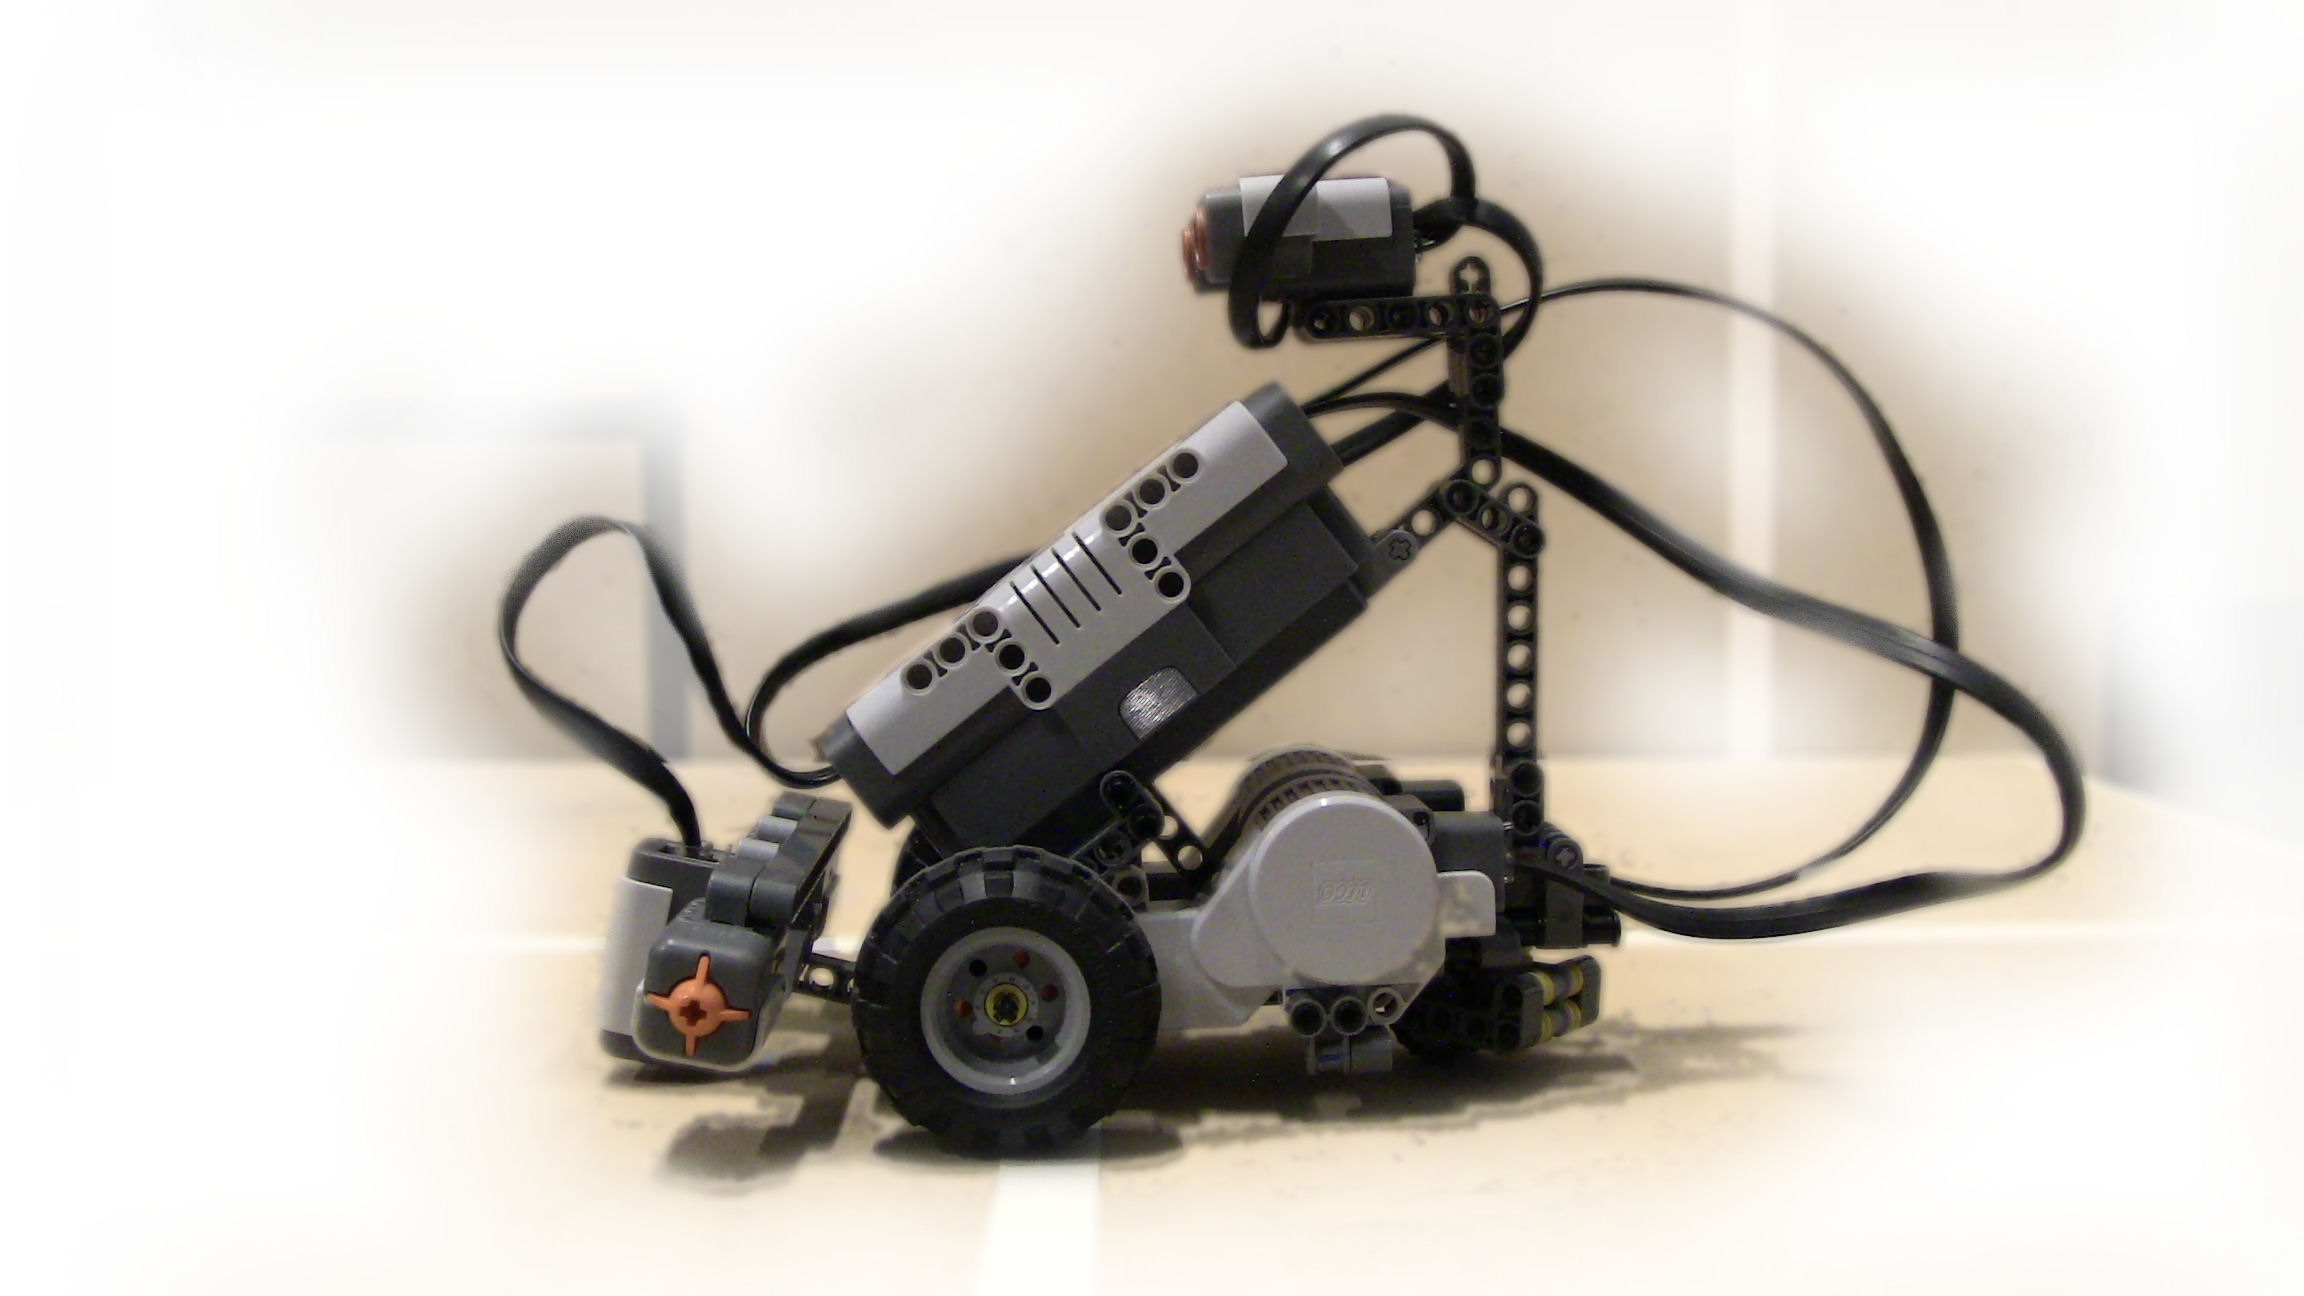
\includegraphics[width=0.8\textwidth]{robotFP2}
    \label{fig:robotFP2}
\end{flushright}
\end{figure}

\newpage
\setcounter{tocdepth}{2}
\tableofcontents

\newpage


% == INLEIDING == %
\section{Inleiding} % 4 ok
\label{ssec:inl}
In het kader van het vak `Probleemoplossen en Ontwerpen: computerwetenschappen' wordt gewerkt rond autonome intelligente robots. Verschillende teams bouwen en programmeren een robot met behulp van LEGO Mindstorms \cite{mindstorms}. Deze robot moet uiteindelijk samen met drie andere robots volledig autonoom \textit{Team Treasure Trek} kunnen spelen.\\

De eerste demonstratie bestaat erin de robot te laten rondrijden in een doolhof. De robot is in staat zijn voorwerp te zoeken en op te pikken terwijl de drie overige robots gesimuleerd worden. Bij het oppikken moet de robot dit laten weten aan zijn teamgenoot. Het is ook mogelijk met vier virtuele robots te werken. De virtuele robots communiceren met elkaar via RabbitMQ.\\


\section{Bouw robot}
\label{ssec:bouwrob}
LEGO Mindstorms \cite{mindstorms} biedt een bouwpakket voor een robot aan. Een NXT-microcomputer laat toe de robot te programmeren. Met behulp van leJOS \cite{leJOS} kan dit in Java.


\subsection{Fysieke bouw}
\label{ssec:fysb}
De robot moet aangepast worden aan de nieuwe opdracht. De robot zal in staat moeten zijn om een voorwerp op te nemen. Er zijn twee veranderingen gebeurt ten opzichte van het eerste semester. De druksensoren aan weerszijde van de lichtsensor zijn weggehaald. Deze stonden er voor tijdens het witte lijn algortime om te detecteren als de robot tegen de muur zou botsen. Deze werden niet geimplementeerd en bleken ook niet nodig te zijn dus zijn deze voor dit semester eruit gehaald. 

De tweede aanpassing is een infraroodsensor bovenop de robot. Deze infraroodsensor dient voor het detecteren van een infrarood balletje. Dit balletje wordt onder de wip geplaatst. Als de wip naar beneden staat zal het balletje verstopt worden door de wip en niet gedetecteerd worden. Hierdoor weet de robot dat de wip naar beneden staat en dat hij doorkan. Als het balletje wel getecteerd wordt, weet de robot dat de wip omhoog staat en dat hij er dus niet over kan. \\

In het begin werd ervoor gekozen om een schep vanachter de robot te monteren om zo het voorwerp op te nemen. Het probleem hiermee is dat de robot dan een te grote lengte krijgt waardoor de robot dus niet meer kan draaien op een tegel zonder te botsen op een muur. \\

Nu is er voor gekozen om het voorwerp langs voor, met een strip van velcro, op te pakken. Het voorwerp ligt het minst in de weg als we het van voor opnemen.




% == ALGORITMES == %
\section{Algoritmes}

Het witte lijn algortime van vorig semester wordt nog steeds behouden. De robot zal zich  dus nog steeds kunnen rechtzetten op witte lijnen.

\subsection{Vinden voorwerp}

Het algoritme voor het vinden van het voorwerp zal grotendeels hetzelfde zijn als het algoritme om een doolhof te doorzoeken. Om het doolhof te doorzoeken gebruiken we het verkenalgoritme, dit moet aangepast worden aan de nieuwe opgave. De mogelijke aanpassingen aan het verkenalgoritme zijn:
\begin{itemize}
\item Aanpassen dat de robot nu ook dead-ends gaat onderzoeken en dat deze prioriteit krijgen.
\item Wanneer ergens mogelijke combinatie straight-deadend gesignaleerd, onmiddellijk naartoe gaan. Kans is groot dat daar het voorwerp ligt.\\
\end{itemize}

\subsection*{Algoritme om zo snel mogelijk naar de andere robot te gaan}
Hierbij dachten we aan het kortste-pad-algoritme. Dit zal wel nog aangepast moeten worden aan zowel draaien als vooruit rijden (draaien was nog niet in rekening gebracht).\\ Er moet ook nog rekening gehouden worden als de andere robot zou wegrijden. De robot mag hierdoor niet in een loop terechtkomen. Er zou moeten gecommuniceerd worden wie naar wie toerijdt, of dat er naar een gezamenlijke tegel moet gereden worden. \\
Als de andere robot zou wegrijden zou er een afstand kunnen bijgehouden worden die dan opnieuw berekent wordt als de afstand niet kleiner wordt.

% == SOFTWARE == %
\section{Software}
\label{secc:softw}

\subsection{RabbitMQ}
\label{secc:RabbMQ}
Via RabbitMG wordt de communicatie met de andere robots verzorgt. RabbitMQ werkt via queue's. .. en nog verdere info

\subsection{GUI}


\subsection{Simulator}
\begin{itemize}
\item Beschrijving van de simulator.
\end{itemize}

\subsection{Software design}
\begin{itemize}
\item Geef hier een klassediagramma en een overzicht van de verschillende methodes.
\end{itemize}

\subsection{\ldots}
\ldots


% == BESLUIT == %
\section{Besluit}



\newpage
\makeappendix

\section{Demo 1}

\subsection{Resultaten}
\ldots

\subsection{Conclusies}
\ldots

\subsection{Oplijsting aanpassingen verslag}
Hier komt een summiere weergave van welke secties uit het vorige verslag gewijzigd werden.





\section{Beschrijving van het proces}
\begin{itemize}
\item Welke moeilijkheden heb je ondervonden tijdens de uitwerking?
\item Welke lessen heb je getrokken uit de manier waarop je het project hebt aangepakt?
\item Hoe verliep het werken in team? Op welke manier werd de teamco\"ordinatie en planning aangepakt?
\end{itemize}


\section{Beschrijving van de werkverdeling}
\begin{itemize}
\item Geef voor elk van de groepsleden aan aan welke delen ze hebben meegewerkt en welke andere taken ze op zich hebben genomen.
\item Rapporteer in tabelvorm hoeveel uur elk groepslid elke week aan het project gewerkt heeft, zowel tijdens als buiten de begeleide sessies. Geef ook totalen per groepslid voor het volledige semester.
\end{itemize}


\section{Kritisch analyse}
\begin{itemize}
\item Maak een analyse van de sterke en zwakke punten van het project. Welke punten zijn vatbaar voor verbetering. Wat zou je, met je huidige kennis, anders aangepakt hebben?
\end{itemize}



\newpage
\bibliographystyle{siam}
\bibliography{biblio.bib}


\end{document}
